\documentclass{article}
\usepackage[final]{NIPS2016}
\usepackage[utf8]{inputenc} % allow utf-8 input
\usepackage[T1]{fontenc}    % use 8-bit T1 fonts
% \usepackage{hyperref}       % hyperlinks
\usepackage{url}            % simple URL typesetting
\usepackage{booktabs}       % professional-quality tables
\usepackage{amsfonts}       % blackboard math symbols
\usepackage{nicefrac}       % compact symbols for 1/2, etc.
\usepackage{microtype}      % microtypography
\usepackage{graphicx}
\usepackage{amsmath}
\usepackage{natbib}

\title{Orc-DeBERTa and Orc-CM: Unsupervised Few-Shot Oracle Character Recognition}

\author{
  Yiqun Wang \\
  School of Data Science \\
  Fudan University \\
  Shanghai, 200433 \\
  \texttt{yiqunwang19@fudan.edu.cn} \\
  \And
  Zichen Cheng \\
  Fudan University \\
  School of Data Science \\
  Shanghai, 200433 \\
  \texttt{zichencheng19@fudan.edu.cn} \\
}

\begin{document}

\maketitle

\begin{abstract}
Oracle characters are the earliest known hieroglyphs in China, and are important for modern archaeology, history, Chinese etymology and calligraphy study, while oracle character recognition is still undeveloped due to the scarcity of oracle bones, the long-tail problem in the usage of characters as well as the high degree of intra-class variance in the shapes of oracle characters.
Since vector form sketch data have been introduced, the oracle character recognition task can be solved either as sequence classification from the perspective of natural language processing (NLP) or image classification from the perspective of computer vision (CV). Therefore, on one hand, we introduce Orc-DeBERTa, which combines the Orc-BERT and the DeBERTa model, and introduce Orc-CM on the other hand.
We fine-tune and test our models on Oracle-FS dataset under self-supervised and few-shot settings, and experiments show that the performance of Orc-DeBERTa exceeds the state-of-the-art model, and that the performance of Orc-CM is not so good as Orc-DeBERTa, which indicates that vector form data can better represent sketch or oracle characters.
\end{abstract}

\section{Introduction}

Oracle characters are the earliest known hieroglyphs in China, which were carved on animal bones or turtle plastrons in purpose of pyromantic divination of weather, state power, warfare and trading to mitigate uncertainty in the Shang dynasty \citep{Oracle}. Oracle characters are important for modern archaeology, history, Chinese etymology and calligraphy study. \citep{Hierachical, Neighbor}

In the past decades, although identification and decipherment for oracle characters have made huge strides, there is still a long way to fully understand the whole writing system. 
So far, more than 150,000 animal bones and turtle shells had been excavated, including approximately 4,500 unique oracle characters, but only about 2,000 of them have been successfully deciphered \citep{OBC306}.
2 main reasons are as follows:

Due to the scarcity of oracle bones and the long-tail problem in the usage of characters as shown in Fig. \ref{fig:distribution}, oracle character recognition suffers from the problem of data limitation and imbalance, thus is a natural few-shot learning problem, which is topical in computer vision and machine learning communities recently. 

Besides, as is shown in Fig. \ref{fig:stroke}, there is a high degree of intra-class variance in the shapes of oracle characters, resulting from the fact that oracle bones were carved by different ancient people in various regions over tens of hundreds of years. As a result, oracle character recognition is a challenging task.

In this paper, we intend to address the problem of oracle character recognition under self-supervision and few-shot settings. More specifically, we will utilize a large-scale unlabeled source data as well as a few labeled training samples for each category to train our model by transferring knowledge.

\section{Related Works}
\label{sec:related}

\paragraph{Vector form sketch data}
Unlike MNIST handwritten digit database \citep{MNIST}, which is in pixel form, oracle data or sketch data are always processed  in vector form \citep{Sketch-BERT}, where we use a 5-dimensional vector to show each point in a sketch:
\begin{equation}
	O = (\Delta x, \Delta y, p_1, p_2, p_3)
	\label{equ:vec}
\end{equation}
In this form, $ \Delta x, \Delta y $ are continuous values, standing for the position offset between two adjacent points,
while $ p_1, p_2, p_3 $ are 0 or 1 and sums to 1, 
where $ p_2 = 1 $ indicates that the point is at the end of a stroke, and $ p_3 = 1 $ indicates that the point is at the end of the whole character.

\paragraph{DeBERTa}
% \citep{GPT} \citep{XLNet}
Since the language representation model BERT is introduced, quite a few works intend to improve it \citep{RoBERTa, DeBERTa}.
DeBERTa is one of them, which implements Disentangled Attention and Enhanced Mask Decoder \citep{DeBERTa, Package}.
On one hand, while BERT’s input is just the sum of token embedding, segment embedding and position embedding, DeBERTa inputs content embedding and position embedding respectively, and the latter represents the relative position between tokens.
On the other hand, since Disentangled Attention only captures relative positions instead of the absolute positions, which is also important, those absolute positions should be incorporated after all the Transformer layers and before the softmax layer for Masked Language Modeling (MLM), so that Transformer layers can make better use of those relative positions, while absolute positions can also play a part in the softmax layer.

\paragraph{Sketch-BERT}
Quite a lot of works have sprung up to process sketch data using deep neural networks. For example, Sketch-a-Net implements 2 novel data augmentation strategies as well as network ensemble fusion strategies to deal with the task of sketch recognition \citep{Sketch-a-Net}; Sketch-RNN studied a generative neural representation for sketches by Long Short Term Memory networks (LSTM) \citep{Sketch-RNN}; Sketch-R2CNN uses an RNN for stroke attention estimation in the vector space, followed by a CNN for 2D feature extraction in the pixel space, also to deal with the task of sketch recognition \citep{Sketch-R2CNN}; TC-Net uses triplet Siamese network and auxiliary classification loss to deal with the task of sketch retrieval \citep{TC-Net}. Among them, Sketch-BERT is the state-of-the-art, which adopts BERT as its backbone \citep{Sketch-BERT}.
It gets sketch embeddings as the sum of point embeddings, position embeddings and stroke embeddings, and pre-trains on a novel self-supervised learning task, sketch Gestalt task, including mask position prediction and mask state prediction.
It can be fine-tuned and tested on downstream tasks, such as sketch recognition, when it adds a \verb|[CLS]| label to the beginning of the sequential data of each sketch, serves as a generic feature extractor of each sketch and adds a standard softmax classification layer at the end.

\paragraph{Orc-BERT}
% \citep{CNN}
As a sub-domain of sketch data processing, quite a lot of works also have sprung up, however pays less attention to deep neural networks. For example, \cite{Hierachical} propose a novel hierarchical representation that combines a Gabor-related low-level representation and a sparse-encoder-related mid-level representation; \citep{Line} uses the line feature to deal with the task of oracle character recognition; \citep{Neighbor} extract features by a convolutional neural network and perform classification by the Nearest Neighbor algorithm also to deal with the task of oracle character recognition; \citep{Detection} present a unified implementation of the Faster R-CNN, SSD, YOLOv3, RFBnet and RefineDet to deal with the the task of oracle character detection; \citep{SSD} extend Single Shot Multibox Detector also to deal with the the task of oracle character detection. Among them, Orc-BERT is the state-of-the-art model in oracle character recognition and is under similar settings as our work \citep{Orc-BERT}.
First, Orc-BERT is pre-trained on a large-scale unlabeled dataset under self-supervision settings by predicting the masked from the visible. Then, convolutional neural network based classifier is trained under few-shot learning settings with Orc-BERT as data augmentor.

\paragraph{CM}
% \citep{MoCo}
Since the oracle character recognition task can be solved either as sequence classification from the perspective of natural language processing (NLP) or image classification from the perspective of computer vision (CV), image inpainting models can also be used as an augmentor. Among all kinds of inpainting models, Globally and Locally Consistent Image Completion (CM) is a typical and relative simple one \citep{CM}, which uses a fully-convolutional neural network, as well as global and local context discriminators 

\section{Approach}

Our model contains 2 parts: augmentor and classifier. When we use Orc-DeBERTa as our augmentor, we can input a masked sketch data and get an augmented image; while when we use Orc-CM as our augmentor, we can input a masked image data and also get an augmented image. Then we can input the augmented data into the classifier, which is based on a pre-trained ResNet-18. The whole structure of our model is shown in figure \ref{fig:whole}.

\begin{figure}[h]
	\centering
	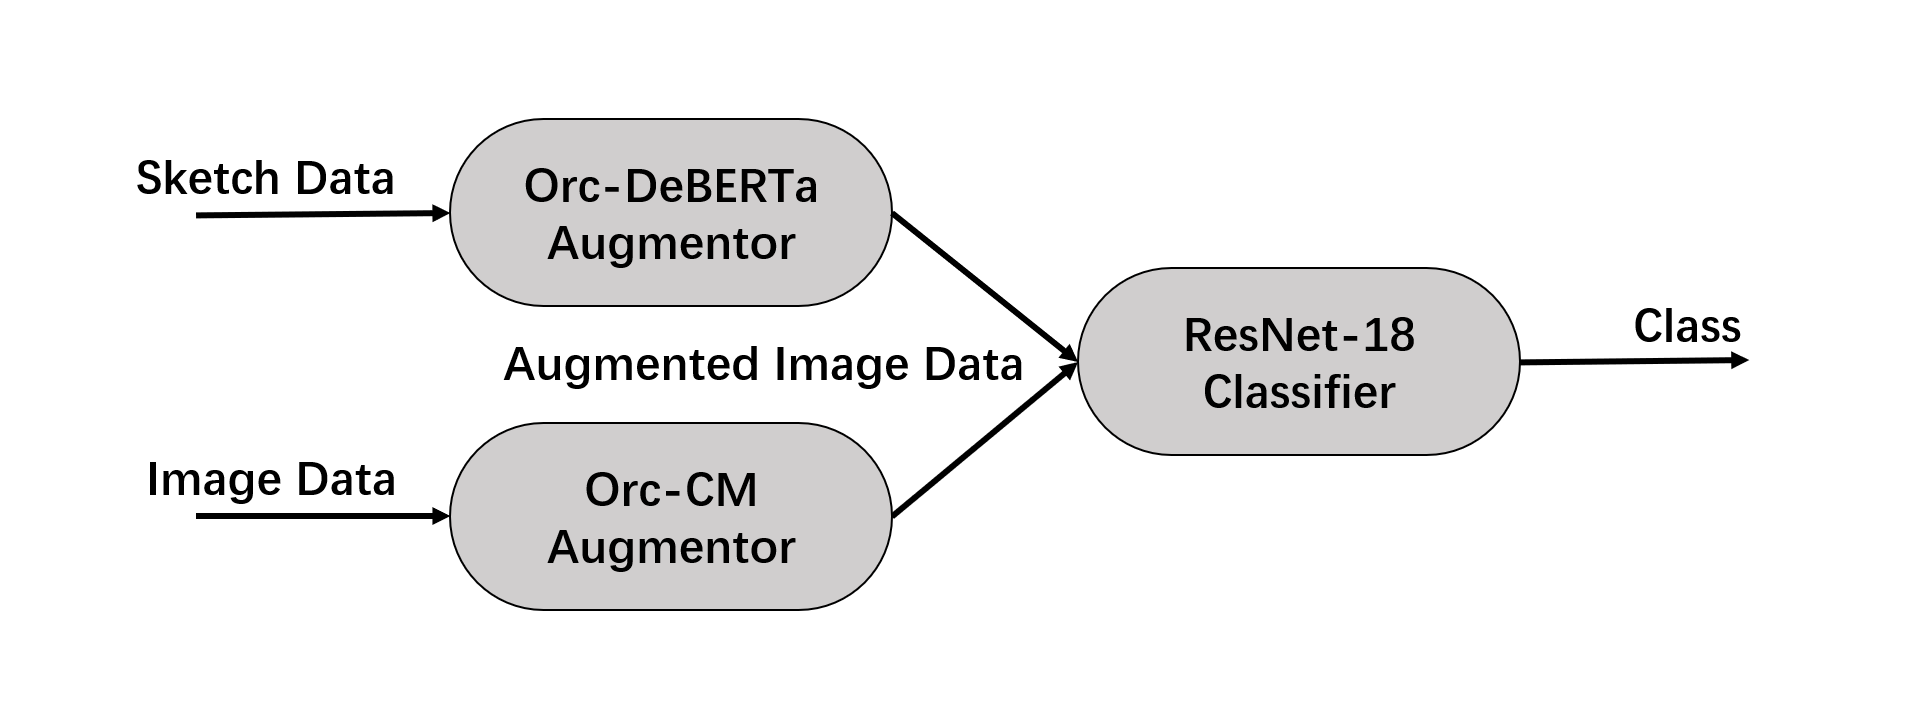
\includegraphics[width=0.75\linewidth]{../Graph/whole.png}
	\caption{The whole structure of our model.}
	\label{fig:whole}
\end{figure}

\subsection{Augmentor}
To increase the volume and diversity of sketches for training, as well as address the challenge of a high degree of intra-class variance in the shapes of sketches, especially under the few-shot settings, data augmentation strategies are quite significant. 
% According to \cite{Sketch-a-Net}, we will not only implement traditional strategies like horizontal and vertical shifts, but also stroke removal and sketch deformation strategies.

% \subsubsection{Stroke Removal}
% \subsubsection{Sketch Deformation}

\subsubsection{Orc-DeBERTa}

When a sketch is inputted into the Orc-DeBERTa, it is first embedded, then encoded and finally outputs an image.

\paragraph{Embedding}
In the DeBERTa \citep{Package}, the input includes the word ID,  the token type ID, the position ID and the mask, while in our Orc-DeBERTa, the word ID is not included. Instead, we use a fully-connected network to create the embedding from the vector from sketch data.

\paragraph{Encoding}
As is mentioned in section \ref{sec:related}, DeBERTa inputs content embedding and position embedding respectively.
More specifically, we denote $ H_i \in R^d $ as the content embedding for a token at position $ i $, and $ P_{i|j} \in R^d  $ as the position embedding to represent the relative position for the token at position $ i $ with the token at position $ j $. 
Then the cross attention score is:
\begin{align*}
	A_{i,j} 
	&= (H_i, P_{i|j}) \cdot (H_j, P_{j|i})^T \\
	&= H_i H_j^T + H_i P_{j|i}^T 
	+ H_j P_{i|j}^T + P_{i|j} P_{j|i}^T
\end{align*}
where the 4 terms stand for content-to-content, content-to-position, position-to-content as well as position-to-position respectively, and the last term can be removed since it doesn't provide much additional information.
To put all $ P_{i|j} $ into a matrix $ P $, we denote $ k $ as the maximum relative distance, and $ \delta (i,j) \in \left[ 0, 2k \right) $ as the relative distance from the token at position $ i $ to the token at position $ j $, where
\begin{equation*}
	\delta (i,j) = 
	\left\{
	\begin{array}{ll}
		0 & i - j \leq k\\
		2k-1 & i - j \geq k \\
		i-j+k & |i - j| < k \\
	\end{array}
	\right.
\end{equation*}
Then the cross attention score is:
\begin{align*}
	\tilde{A_{i,j}}
	&= Q^c_i {K^c_j}^T 
	+ Q^c_i {K^r_{\delta (i,j)}}^T 
	+ K^c_j {Q^r_{\delta (j,i)}}^T
\end{align*}
where
\begin{align*}
	Q^c &= H W_{q,c} & K^c &= H W_{k,c} \\
	Q^r &= P W_{q,r} & K^r &= P W_{k,r} 
\end{align*}
are projected matrices and $ W_{q,c} \ W_{k,c} \ W_{q,r} \ W_{k,r}$ are projection matrices.
Finally, the output of self-attention operation is
$ H_o = softmax(\frac{\tilde{A}}{\sqrt{3d}}) V^c $
where $ V^c = H W_{v,c} $.

\paragraph{Reconstruction}
After encoding, we use a fully-connected network to further reconstruct the information and output an image.

\subsubsection{Orc-CM}

\subsection{Classifier}

We use pre-trained ResNet-18 as the classifier \citep{ResNet}, where the output is the probability of the 200 classes.

\section{Experiment}

\subsection{Dataset}

\paragraph{Oracle-50K}
In this dataset, labeled oracle character samples are collected  from three data sources using different strategies \citep{Orc-BERT}. There are 2668 unique characters and 59081 images in total. Besides, as is shown in Fig. \ref{fig:distribution}, there exists a long-tail distribution of oracle character samples in Oracle-50K. Therefore, oracle character recognition is a natural few-shot learning problem.

\begin{figure}[h]
	\centering
	\includegraphics[width=0.75\linewidth]
	{../Papers/Distribution.png}
	\caption{The distribution of oracle character samples in dataset Oracle-50K.}
	\label{fig:distribution}
\end{figure}

\paragraph{Oracle-FS}
Based on Oracle-50K and other collected ancient Chinese character images, \cite{Orc-BERT} created a few-shot oracle character recognition dataset, Oracle-FS, including 276,031 images, under three different few-shot settings. 
Specifically, under the $k$-shot setting, there are 200 classes, with $k$ training samples and 20 test ones per class, where k can be 1, 3 and 5.
Besides, since the stroke orders of Chinese characters contain a lot of information, for which people can usually recognize a character correctly even if it is incomplete, Oracle-FS includes both pixel and vector format data.
Although the stroke orders of oracle characters have been lost in history, there are two fundamental facts: 1) oracle writing is ancestral to modern Chinese script; 2) the modern Chinese writing system is in a left-to-right then top-to-bottom writing order, so assuming oracle character writing is in the same order and using existing approximation algorithm \citep{Handwriting}, character images in pixel format can be converted to data in vector format.  
Nevertheless, due to 3 failure cases during approximation algorithm, the number of source samples in vector format are 276,028.

\begin{figure}[h]
	\centering
	\includegraphics[width=0.75\linewidth]
	{../Papers/Stroke.png}
	\caption{Examples of oracle character images and corresponding stroke data.}
	\label{fig:stroke}
\end{figure}

\subsection{Data Pre-process}

\paragraph{Pixel Form Image Data}
In Oracle-FS dataset, all images are gray-scale ones, whose pixel values ranging from 0 to 255. Since pixel value 255 means the white background, we get all pixel values be divided by 256 and be minus by 1.

\paragraph{Vector Form Sketch Data}
First, the vector form sketch data in equation \ref{equ:vec} is simplified into:
\begin{equation*}
	O = (\Delta x, \Delta y, p_2 + p_3) 
\end{equation*} 
since $ p_1 = 1 $ at most times.
In Oracle-FS dataset, it satisfies:
\begin{align*}
	\Delta x &\in [-49, 49] \\
	\Delta y &\in [-49, 49] \\
	p_2 + p_3 &\in \{0, 1\}
\end{align*}
To normalize the data, we get:
\begin{equation*}
	\tilde{O} = 
	(\frac{\Delta x}{49}, \frac{\Delta y}{49},	p_2 + p_3) 
\end{equation*} 
Finally, to get same length for all sketch data, we pad them with $(0, 0, 2)$.

\subsection{Hyper-parameters}

During training, the number of epochs is 200, the batch size is 8, the optimizer is Adam, and the learning rate is 0.0001 and 0.001 for augmentor pre-training and classifier training respectively.

As for the structure of the Orc-DeBERTa augmentor, as what Orc-BERT did, the max input length of stroke is 300, the hidden size is 128 and the number of weight-sharing Transformer layers is 8. The embedding and reconstruction networks are fully-connected with structure of 64-128-128 and 128-128-64-5 respectively. The size of augmented images is $ 50 \times 50 $, and becomes $ 224 \times 224 $ for the classifier.

As for the mask probability, as what Orc-BERT did, during pre-training, the probability is 15\%; during augmentation, 80 different mask probability is implemented to generate diverse augmented data, ranging from 0.1 to 0.5, uniformly spacing.

\subsection{Results}

Our results are shown in table \ref{tab:results}.

\begin{table}[h]
	\centering
	\caption{The results of our experiments}
	\begin{tabular}{cccc}
		\toprule
		Setting & No DA & Orc-DeBERTa & Orc-CM \\
		\midrule
		1-shot & 0.40100 &  &  \\
		3-shot & 0.65675 &  &  \\
		5-shot & 0.76375 &  &  \\
		\bottomrule
	\end{tabular}
	\label{tab:results}
\end{table}

\section{Conclusion}

\bibliographystyle{unsrtnat}
\bibliography{Report}

\end{document}
